\newpage
\section{Права пользователей}

\subsection{Постановка задачи}
В работе проверяется разграничение доступа к базе данных для двух пользователей.
Пользователь \textbf{А} имеет право только просматривать таблицу
\texttt{car\_stats}. Пользователь \textbf{Б} может
просматривать и изменять исходные таблицы \texttt{car}, \texttt{alert\_event}
и \texttt{parking\_session}, а также таблицу \texttt{parking\_zone}, удаление
которой приводит к каскадному удалению связанных сессий. Изменения этих таблиц должны отражаться в
\texttt{car\_stats} благодаря ранее созданным триггерам.

Пользователю \textbf{А} не предоставляются права на исходные таблицы и изменение данных.
Пользователь \textbf{Б} также не получает прямого права читать или изменять
\texttt{car\_stats}; таблицу статистики читает пользователь \textbf{А}. Пользователь \textbf{Б}
получает права на чтение и выполнение операций
\texttt{INSERT}, \texttt{UPDATE} и \texttt{DELETE} в исходных таблицах, но не
получает прямого доступа к \texttt{car\_stats}.

\subsection{Назначение прав доступа}
В листинге~\ref{lst:user-privileges} приведён шаблон назначения прав.
Перед запуском необходимо заменить имена ролей и пароли на используемые в
учебной базе данных. Команды создания ролей выполняются администратором БД.

\begin{lstlisting}[style=sqlstyle, caption={Создание пользователей и назначение прав}, label={lst:user-privileges}]
CREATE USER user_a WITH PASSWORD '123';
CREATE USER user_b WITH PASSWORD '123';

GRANT CONNECT ON DATABASE db TO user_a, user_b;
GRANT USAGE ON SCHEMA public TO user_a, user_b;

-- пользователь А читает только таблицу car_stats
GRANT SELECT ON car_stats TO user_a;

-- пользователь Б читает и изменяет исходные таблицы, но не имеет прямого доступа к car_stats
GRANT SELECT, INSERT, UPDATE, DELETE 
ON TABLE car, alert_event, parking_session, parking_zone
TO user_b;

-- для пользователя Б разрешаем автоинкрементные id
GRANT USAGE, SELECT ON SEQUENCE
	car_car_id_seq, 
	alert_event_alert_event_id_seq, 
	parking_session_parking_session_id_seq, 
	parking_zone_parking_zone_id_seq
TO user_b;

ALTER FUNCTION car_stats_change() SECURITY DEFINER  SET search_path = public;

ALTER FUNCTION alert_event_stats_change() SECURITY DEFINER SET search_path = public;

ALTER FUNCTION parking_session_stats_delete() SECURITY DEFINER SET search_path = public;
\end{lstlisting}

Пользователь А получает право \texttt{SELECT} только на \texttt{car\_stats};
пользователь Б получает права чтения и изменения таблиц, влияющих на
статистику. Функции триггеров должны исполняться с правами владельца функции,
иначе PostgreSQL проверяет право пользователя Б обновить \texttt{car\_stats}
и может отклонить операцию.

\subsection{Проверка прав пользователей}
Проверка выполняется в двух отдельных текстовых консолях, подключённых к одной
базе данных: левая консоль работает от имени пользователя А, правая — от имени
пользователя Б. Сначала запрос № 1 выполняется в консоли пользователя А. Затем пользователь Б
выполняет запросы на добавление, изменение и удаление данных.
После каждого успешно завершённого изменения пользователь А повторно выполняет
запрос к \texttt{car\_stats} и видит обновлённые значения.

Для проверки удаления сначала следует сохранить исходную строку статистики и
выполнить удаление тестовой записи, а затем проверить результат. Тестовые
операции нужно выполнять на данных, которые разрешено изменять. Если сценарий
проверяется внутри транзакции, пользователь Б должен выполнить \texttt{COMMIT}
перед тем, как пользователь А проверит новое состояние в другой консоли.

В таблице~\ref{tab:user-privileges-tests} приведён шаблон протокола проверки.
Вместо текста в квадратных скобках следует внести фактический SQL-запрос,
ответ СУБД или наблюдавшийся результат. Идентификаторы и значения для тестовых
записей нужно выбрать по существующим данным базы.

\subsubsection{Последовательность проверки в двух консолях}
На рисунках ниже следует разместить снимки обеих консолей рядом. В левой
консоли выполняются команды от имени пользователя А, в правой — от имени
пользователя Б. Перед началом выбирается существующий \texttt{car\_id}, а для
вставки события — допустимые значения \texttt{alert\_event\_type\_id} и
\texttt{status\_id}. Все изменения выполняются для тестовых данных.

\paragraph{Шаг 1. Исходное состояние.}
Пользователь А читает статистику выбранного автомобиля. Полученное значение
\texttt{alert\_count} записывается как исходное.
\begin{lstlisting}[style=sqlstyle]
-- Левая консоль, пользователь А
SELECT car_id, alert_count
FROM car_stats
WHERE car_id = <car_id>;
\end{lstlisting}
На снимке~\ref{fig:access-before} показать левую консоль с исходным
значением статистики и правую консоль, подключённую как пользователь Б.

\begin{figure}[H]
    \centering
    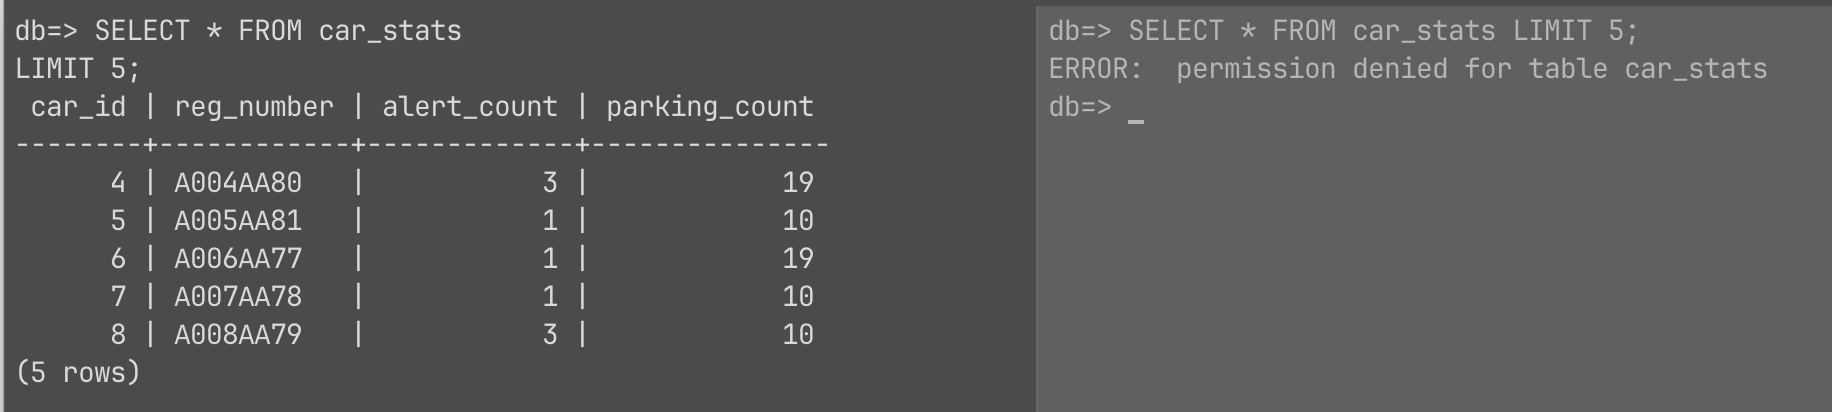
\includegraphics[width=0.8\linewidth]{myPhoto/access-before.png}
    \caption{Исходное состояние таблицы статистики в консоли пользователя А}}
    \label{fig:access-before}
\end{figure}

Также проверим что пользователь Б может прочитать исходную таблицу \texttt{car}.
\begin{figure}[H]
    \centering
    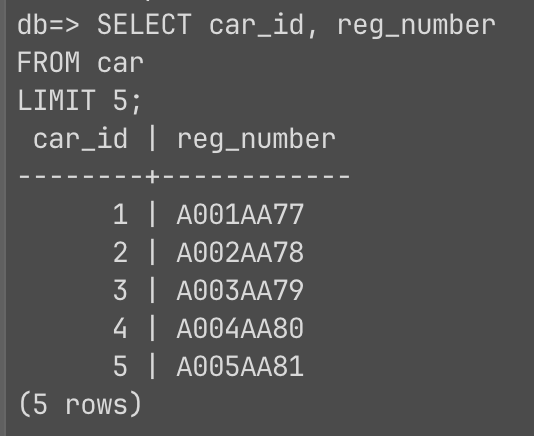
\includegraphics[width=0.5\linewidth]{myPhoto/b_car.png}
    \caption{Пользователь Б может прочитать исходную таблицу \texttt{car}}
    \label{fig:b_car}
\end{figure}


\paragraph{Шаг 2. Вставка события пользователем Б.}
Пользователь Б добавляет тревожное событие и фиксирует транзакцию командой
\texttt{COMMIT}. В ответе сохраняется выданный идентификатор события.
\begin{lstlisting}[style=sqlstyle]
-- Правая консоль, пользователь Б
INSERT INTO alert_event (
    car_id, alert_event_type_id, status_id, description
)
VALUES (
    <car_id>, <тип_события>, <статус>, 'Проверка прав пользователей'
)
RETURNING alert_event_id;
COMMIT;
\end{lstlisting}
На снимке~\ref{fig:access-check-insert} показать выполненную вставку и
полученный идентификатор в правой консоли.

\begin{figure}[H]
    \centering
    \fbox{\parbox[c][4cm][c]{0.9\textwidth}{\centering
    Место для снимка двух консолей: успешная вставка пользователя Б\newline
    Файл после заполнения: \texttt{myPhoto/access-insert.png}}}
    \caption{Добавление тревожного события пользователем Б}
    \label{fig:access-check-insert}
\end{figure}

\paragraph{Шаг 3. Проверка результата и ограничений.}
Пользователь А повторно выполняет запрос из шага 1. Значение
\texttt{alert\_count} должно увеличиться на единицу. Пользователь Б может
прочитать исходную таблицу \texttt{alert\_event}, но попытка читать
\texttt{car\_stats} должна завершиться отказом в доступе.
\begin{lstlisting}[style=sqlstyle]
-- Левая консоль, пользователь А: статистика обновилась
SELECT car_id, alert_count
FROM car_stats
WHERE car_id = <car_id>;

-- Правая консоль, пользователь Б: свою исходную запись он видит
SELECT alert_event_id, car_id
FROM alert_event
WHERE alert_event_id = <id_события>;

-- Но прямое чтение статистики ему запрещено
SELECT * FROM car_stats WHERE car_id = <car_id>;
\end{lstlisting}
На снимке~\ref{fig:access-check-after-insert} показать увеличение счётчика в
левой консоли и отказ в прямом чтении \texttt{car\_stats} в правой консоли.

\begin{figure}[H]
    \centering
    \fbox{\parbox[c][4cm][c]{0.9\textwidth}{\centering
    Место для снимка двух консолей: новое значение счётчика у А; отказ SELECT у Б\newline
    Файл после заполнения: \texttt{myPhoto/access-after-insert.png}}}
    \caption{Обновление статистики и запрет прямого чтения для пользователя Б}
    \label{fig:access-check-after-insert}
\end{figure}

\paragraph{Шаг 4. Проверка удаления.}
Сначала пользователь А пытается удалить добавленное событие. СУБД должна
отклонить запрос из-за отсутствия права \texttt{DELETE}. Затем пользователь Б
удаляет тестовое событие по полученному на шаге 2 идентификатору и выполняет
\texttt{COMMIT}. После этого пользователь А снова читает статистику: значение
\texttt{alert\_count} должно вернуться к исходному.
\begin{lstlisting}[style=sqlstyle]
-- Левая консоль, пользователь А: ожидается отказ в доступе
DELETE FROM alert_event
WHERE alert_event_id = <id_события>;

-- Правая консоль, пользователь Б: удаление разрешено
DELETE FROM alert_event
WHERE alert_event_id = <id_события>;
COMMIT;

-- Левая консоль, пользователь А: счётчик вернулся к исходному
SELECT car_id, alert_count
FROM car_stats
WHERE car_id = <car_id>;
\end{lstlisting}
На снимке~\ref{fig:access-check-delete} показать отказ пользователю А,
успешное удаление пользователем Б и исходное значение счётчика после удаления.

\begin{figure}[H]
    \centering
    \fbox{\parbox[c][4cm][c]{0.9\textwidth}{\centering
    Место для снимка двух консолей: отказ DELETE у А, успешный DELETE у Б,\newline
    восстановившийся счётчик у А\newline
    Файл после заполнения: \texttt{myPhoto/access-delete.png}}}
    \caption{Проверка удаления события пользователями А и Б}
    \label{fig:access-check-delete}
\end{figure}

\paragraph{Шаг 5. Обращение к неразрешённой таблице.}
В обеих консолях выполняется запрос к таблице \texttt{alert\_event\_type},
для которой права не выдавались. Ожидаемый результат — отказ обоим пользователям.
Снимок двух консолей добавить на рисунок~\ref{fig:access-check-denied}.

\begin{figure}[H]
    \centering
    \fbox{\parbox[c][4cm][c]{0.9\textwidth}{\centering
    Место для снимка двух консолей: отказ SELECT из \texttt{alert\_event\_type}\newline
    Файл после заполнения: \texttt{myPhoto/access-denied.png}}}
    \caption{Отказ обоим пользователям при обращении к неразрешённой таблице}
    \label{fig:access-check-denied}
\end{figure}


\begin{longtable}{|c|p{7.0cm}|p{3.0cm}|p{3.0cm}|}
\caption{Результаты проверки прав пользователей}\label{tab:user-privileges-tests}\\
\hline
№ & SQL-запрос & Реакция пользователя А & Реакция пользователя Б \\
\hline
\endfirsthead
\hline
№ & SQL-запрос & Реакция пользователя А & Реакция пользователя Б \\
\hline
\endhead
1 & \texttt{SELECT * FROM car\_stats LIMIT 5;} & Успешно: вывод строк статистики & Отказ: нет права на \texttt{car\_stats} \\
\hline
2 & \texttt{INSERT INTO alert\_event (...)}\newline [подставить допустимые значения] & Отказ: нет права на \texttt{alert\_event} & Успешно: [указать ID добавленной записи] \\
\hline
3 & \texttt{UPDATE car SET reg\_number = ... WHERE car\_id = ...;}\newline [тестовый автомобиль] & Отказ: нет права на \texttt{car} & Успешно: [указать результат] \\
\hline
4 & \texttt{DELETE FROM parking\_session WHERE parking\_session\_id = ...;}\newline [тестовая сессия] & Отказ: нет права на \texttt{parking\_session} & Успешно: [указать результат] \\
\hline
5 & \texttt{SELECT * FROM car\_stats WHERE car\_id = ...;}\newline [проверить результат изменения пользователя Б] & Успешно: [указать новые счётчики] & Отказ: нет права на \texttt{car\_stats} \\
\hline
6 & \texttt{SELECT * FROM alert\_event\_type LIMIT 1;} & Отказ: нет права на \texttt{alert\_event\_type} & Отказ: нет права на \texttt{alert\_event\_type} \\
\hline
\end{longtable}

\subsection{Описание результатов проверки}
Запрос № 1 подтвердил, что пользователь А может читать таблицу
\texttt{car\_stats}. Запросы № 2--4 проверили операции изменения исходных
таблиц пользователем Б и отказ в этих операциях для пользователя А.
После фиксации изменений запрос № 5 подтвердил, что результат работы триггеров
виден пользователю А, при этом пользователь Б не имеет прямого права читать
\texttt{car\_stats}. Запрос № 6 проверил обращение к неразрешённой таблице:
обоим пользователям отказано, так как таблица \texttt{alert\_event\_type} не
входит в список разрешённых для них таблиц.
Фактические сообщения СУБД и значения статистики следует вписать в таблицу
после выполнения программы назначения прав и тестовых запросов.
